\section{Summary}

Between 13\textsuperscript{th} July and 19\textsuperscript{th} August 2012, Imperial College Caving Club had
twenty-six members participate in the Sledi Vetra 2012 expedition to \passage{Tolminski Migovec},
Slovenia.

There were two major aims for this expedition. One was the continued
exploration of \passage{Vrtnarija}, where considerable efforts in 2010 and
2011 had led to the discovery of 4.4 km of mainly horizontal passage,
all below 500 m in depth. The other was to connect \passage{Vrtnarija} with
\passage{Sistem Migovec} (which ICCC first started exploring in 1994),
thus forming the longest cave system in Slovenia. At the start of the
expedition, \passage{Vrtnarija} was 11025 m long and 888 m deep, and the
smallest separation between \passage{Kavkna Jama} (\passage{M2} entrance in
\passage{SysMig}) and \passage{Vrtnarija} was 4 m (±30 m survey error).

In addition, an enduring desire to understand the caves of \passage{Migovec} meant
that surface work in \passage{Area K}, \passage{Area S} and \passage{Area N} (north of \passage[mountain]{Kuk}) was also a major
consideration during the expedition.

\begin{marginfigure}
\checkoddpage \ifoddpage \forcerectofloat \else \forceversofloat \fi
\centering
 \frame{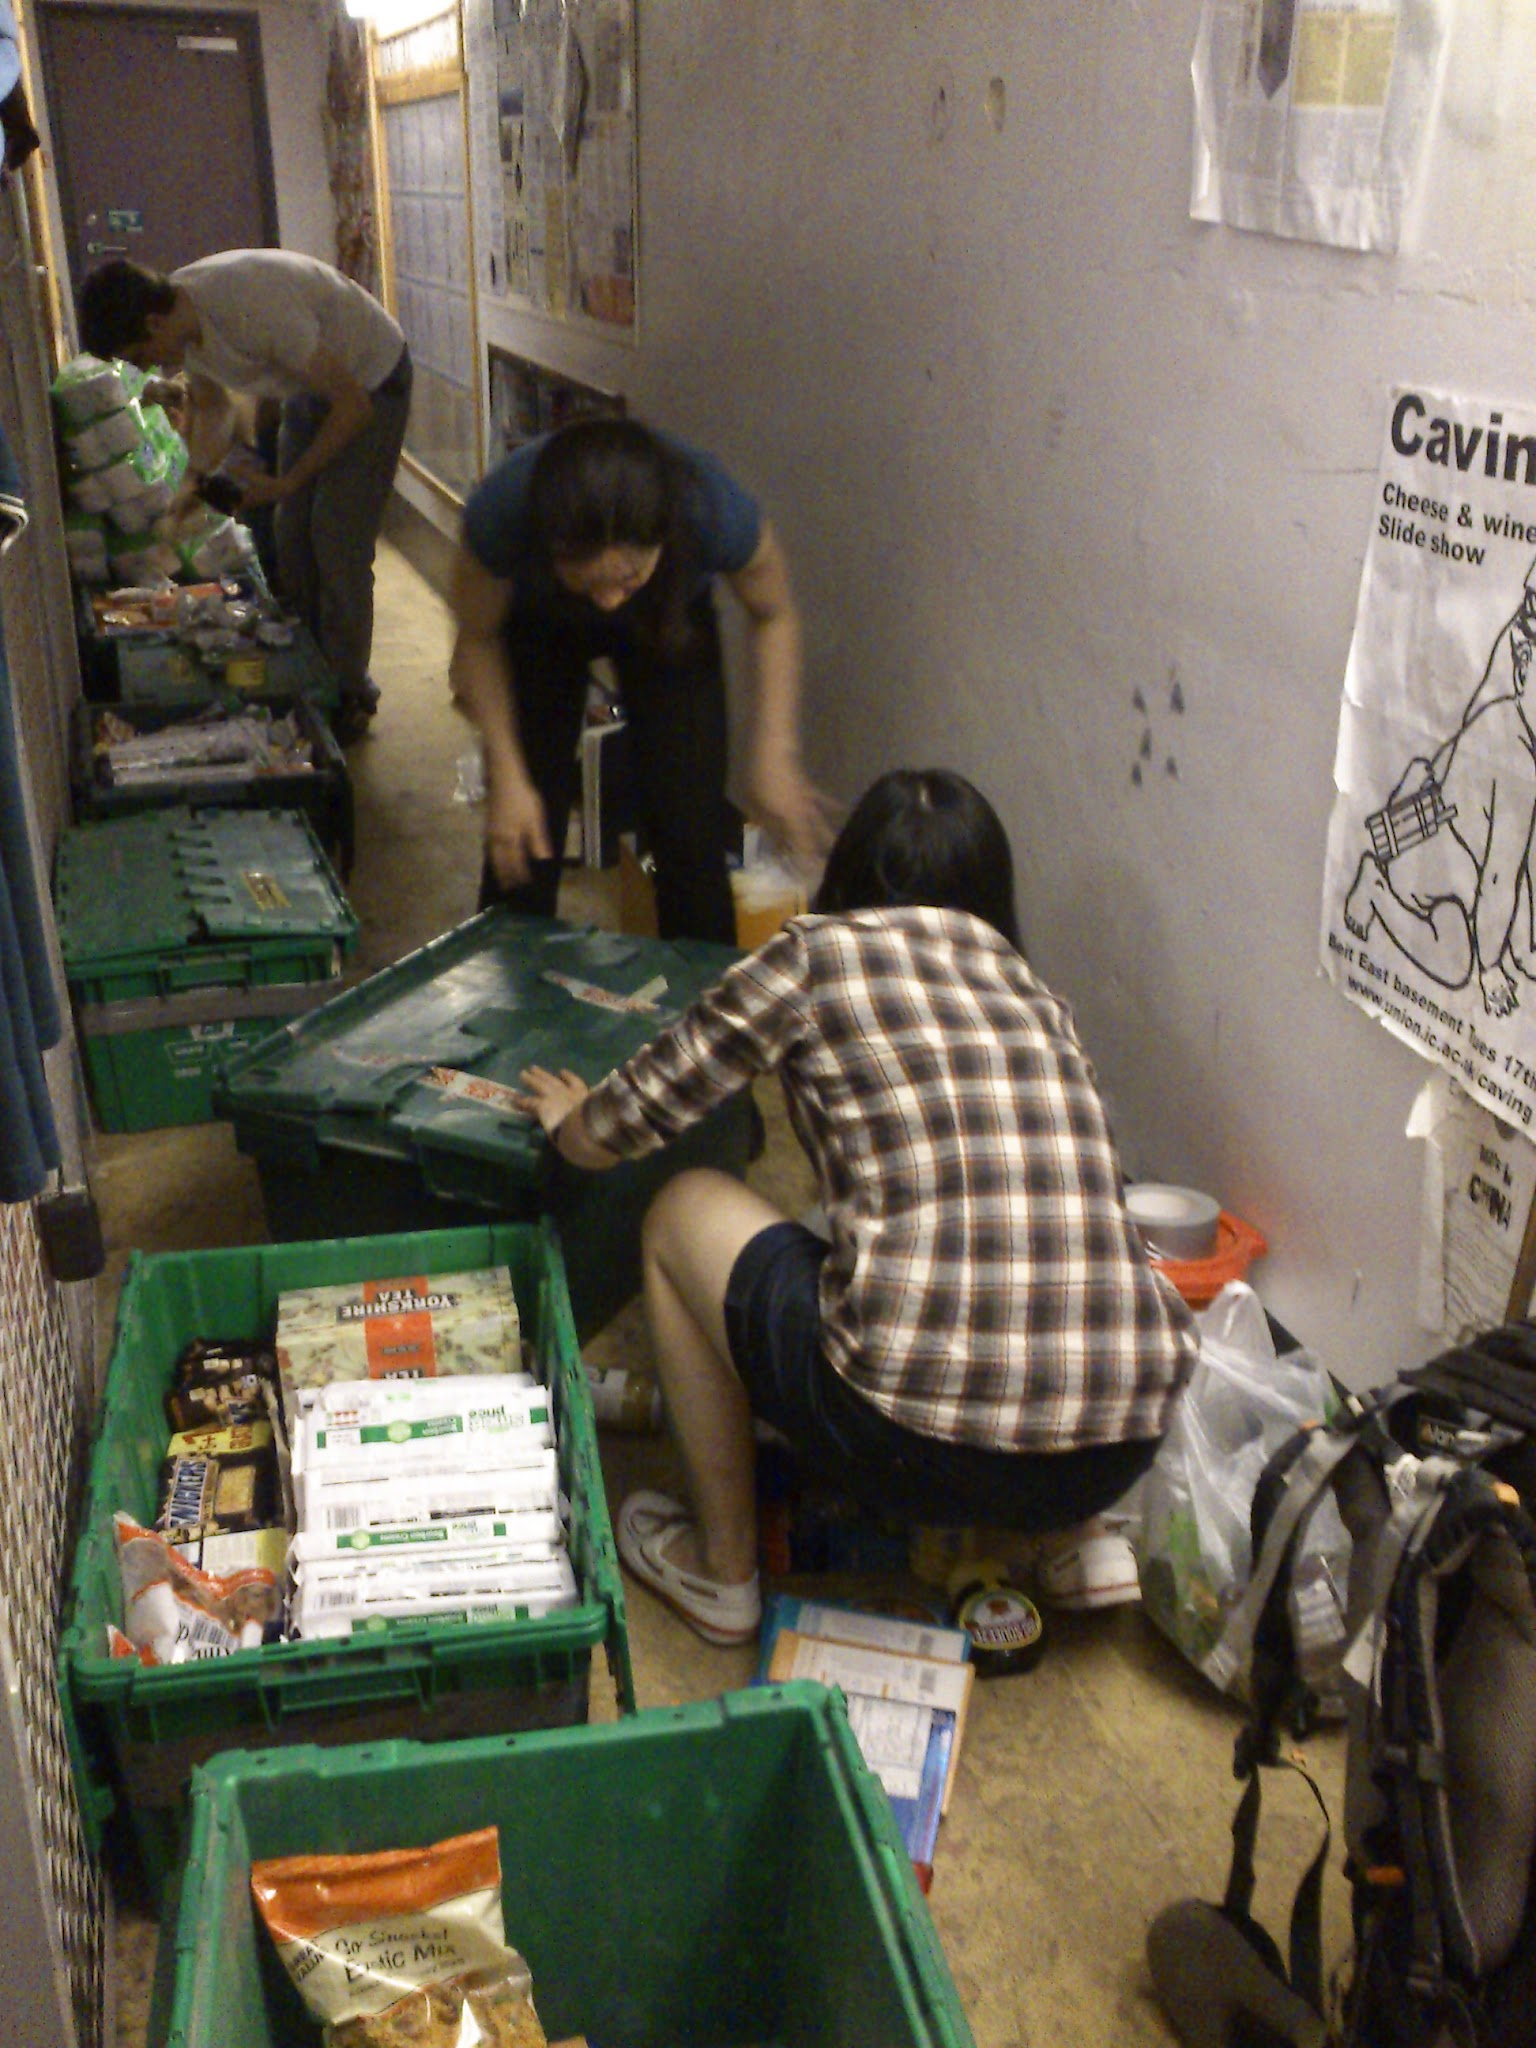
\includegraphics[width=\linewidth]{2012/summary/2012-07-07-1459JarvistMooreFrost-DSC_0260--orig.jpg}} 
 \caption{With 6 days to go, the LIDL / ASDA raid was a success, with food sorted away into crates in preparation for the final loading of the minibus. \pic{Jarvist Frost}}
 \label{crate pack}
\end{marginfigure}

A large and strong UK team, and a longer-than-usual expedition (five
weeks instead of four) meant that we had sufficient manpower and time to
achieve all expedition aims.


\begin{pagefigure}
\checkoddpage \ifoddpage \forcerectofloat \else \forceversofloat \fi
   \centering
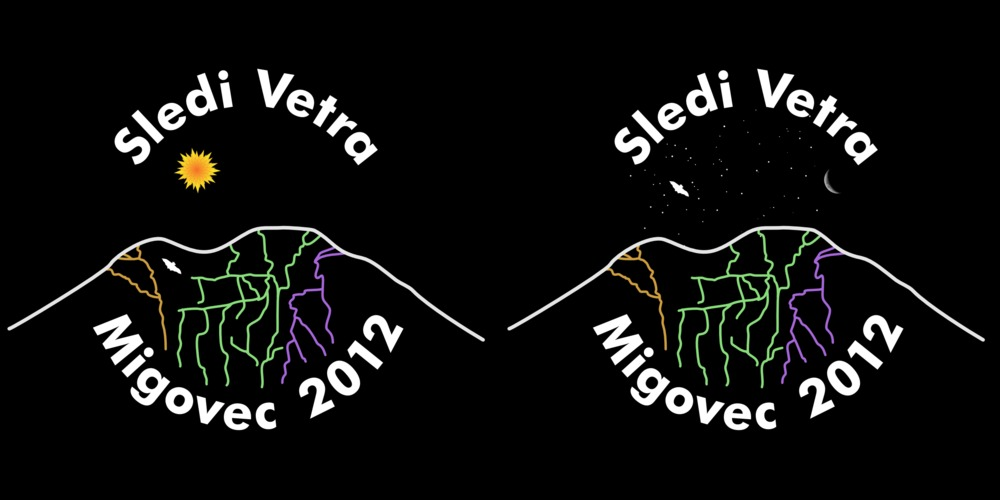
\includegraphics[width = \textwidth]{2012/summary/2012-01-29_print_res_both-png-scaled-1000.jpg}
\caption{The two logos (day and night) for the Sledi Vetra expedition. \pen{Jarvist Frost}} \label{2012 logos}
\end{pagefigure}


As in previous expeditions ('03, '10, '11), an underground camp (Camp
\passage{X-Ray}) was set up at -550 m in \passage{Vrtnarija} to facilitate
further exploration of the deep leads. Eighteen people from the UK and
six Slovenes from the local JSPDT club spent nights at \passage{X-Ray} for
a total of 90 people-nights. This included three first-year cavers, all
of whom contributed significantly to exploration. All but one pushing
trips were done on overnight camps, with almost all successful
exploration occurring below 500 m.

Three separate trips were made to \passage{Kavkna Jama} in an attempt to
forge the connection between \passage{SysMig} and \passage{Vrtnarija}. Though an
acoustic connection was made when parties sent down \passage{Captain Kangaroo} in
\passage{Vrtnarija} could hear the sound of drilling and hammering
occurring in \passage{Kavkna Jama}, the actual physical connection was
elusive. Somewhat unexpectedly, the connection was instead made in a
completely separate area of the cave when \passage{Dreams for the Soul}, a
phreatic passage off \passage{Queen's Bedchamber} in \passage{Vrtnarija},
dropped into \passage{Waterloo} in \passage{SysMig} (all at $\approx$ -600 m).

\begin{marginfigure}
\checkoddpage \ifoddpage \forcerectofloat \else \forceversofloat \fi
\centering
 \frame{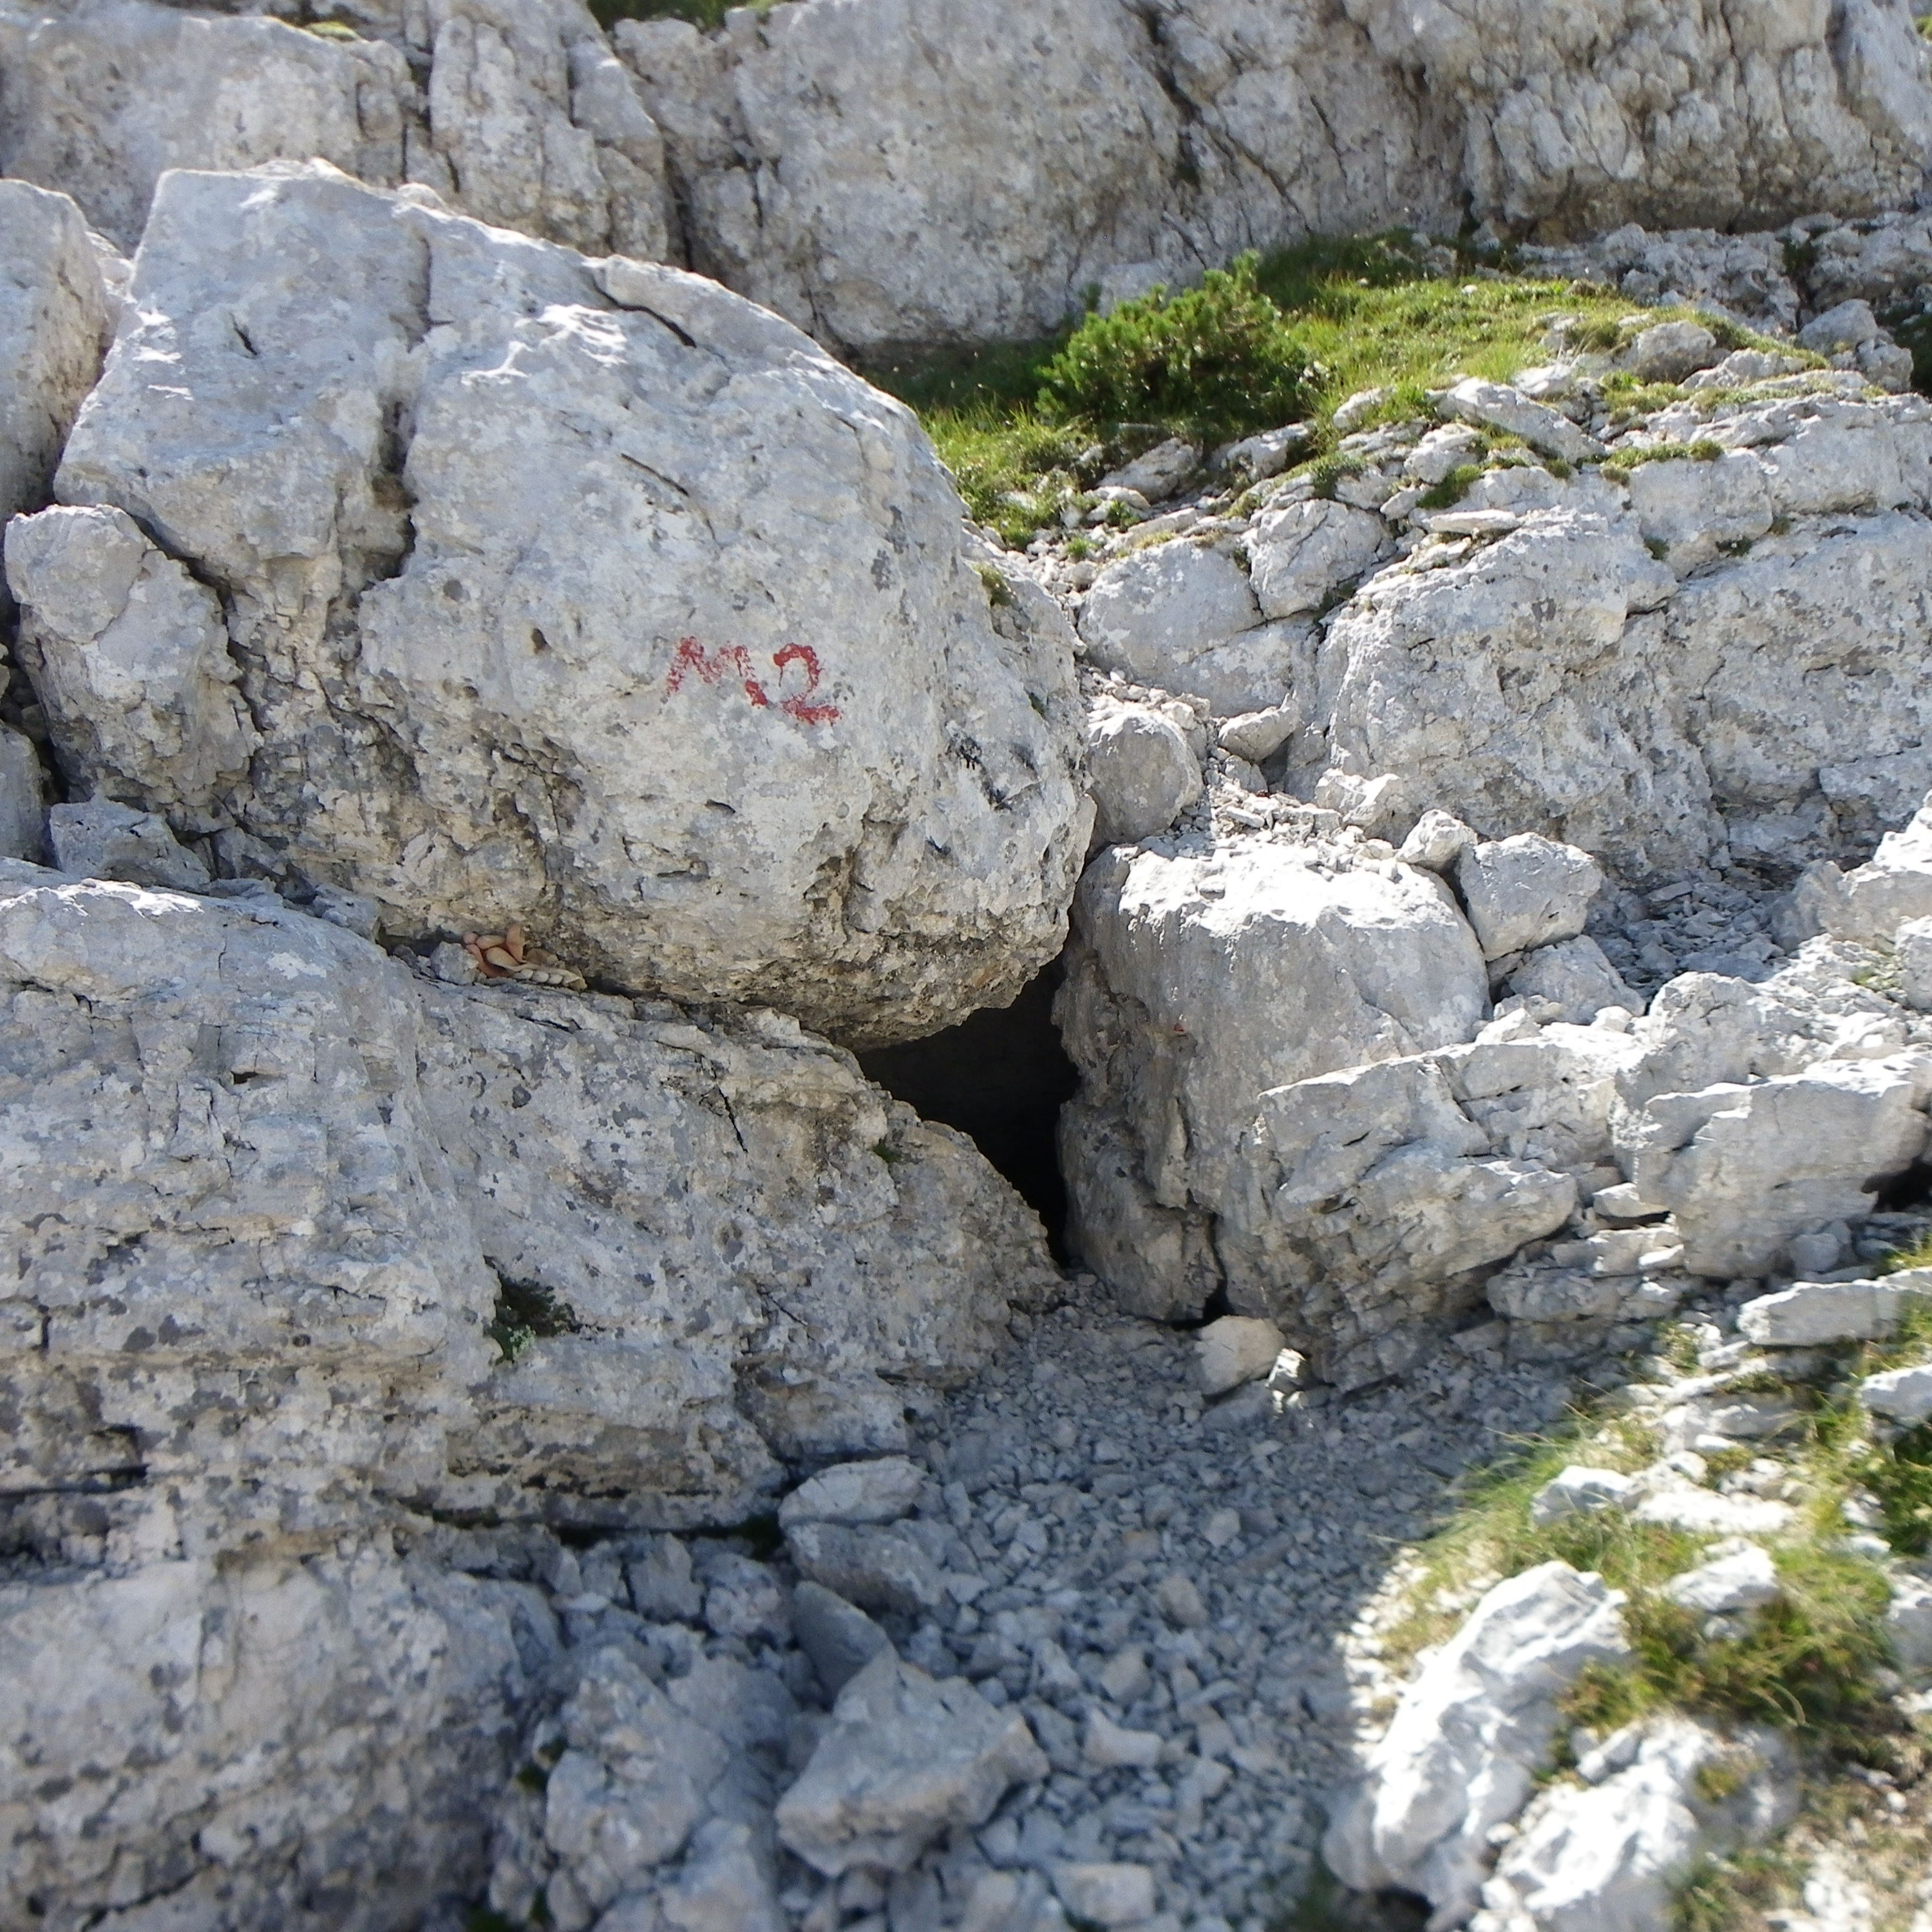
\includegraphics[width=\linewidth]{2012/summary/2012-08-08-15.08.58-Rhys Tyers-Pentax X90-IMGP3352--orig.jpg}} 
 \caption{The unassuming entrance to \passage{M2}, \passage{Kavkna Jama}. \pic{Rhys Tyers}}
 \label{m2 entrance}
\end{marginfigure}

Aided by perfect weather for much of the expedition, surface work was
carried out by cavers in between underground camps. Most of it was
concentrated in \passage{Areas K and N}. Two pitches were dropped in \passage{N9} (a.k.a.
\passage{Kuk Pot}), and the cave was pushed to a depth of 25 metres with 29 metres of cave passage.

Many entrances in \passage{Area K} were also re-visited. \passage{K2} remains the most
promising, while digging went on in \passage{K19}.

In all we discovered 2703 m of new cave passage taking \passage{Vrtnarija}
to 13728 m long and 900 m deep. Thanks to the connection, the combined
\passage{System Migovec} is now 25592 m long and 973 m deep, with the deepest
point being \passage{Watership Down} in \passage{Vrtnarija}, found during this
year's expedition. This makes \passage{SysMig} the longest cave system in
Slovenia, displacing the famous \passage{Postojna Jama} as the previous record
holder at 20190 m.

\begin{pagefigure}
\checkoddpage \ifoddpage \forcerectofloat \else \forceversofloat \fi
   \centering
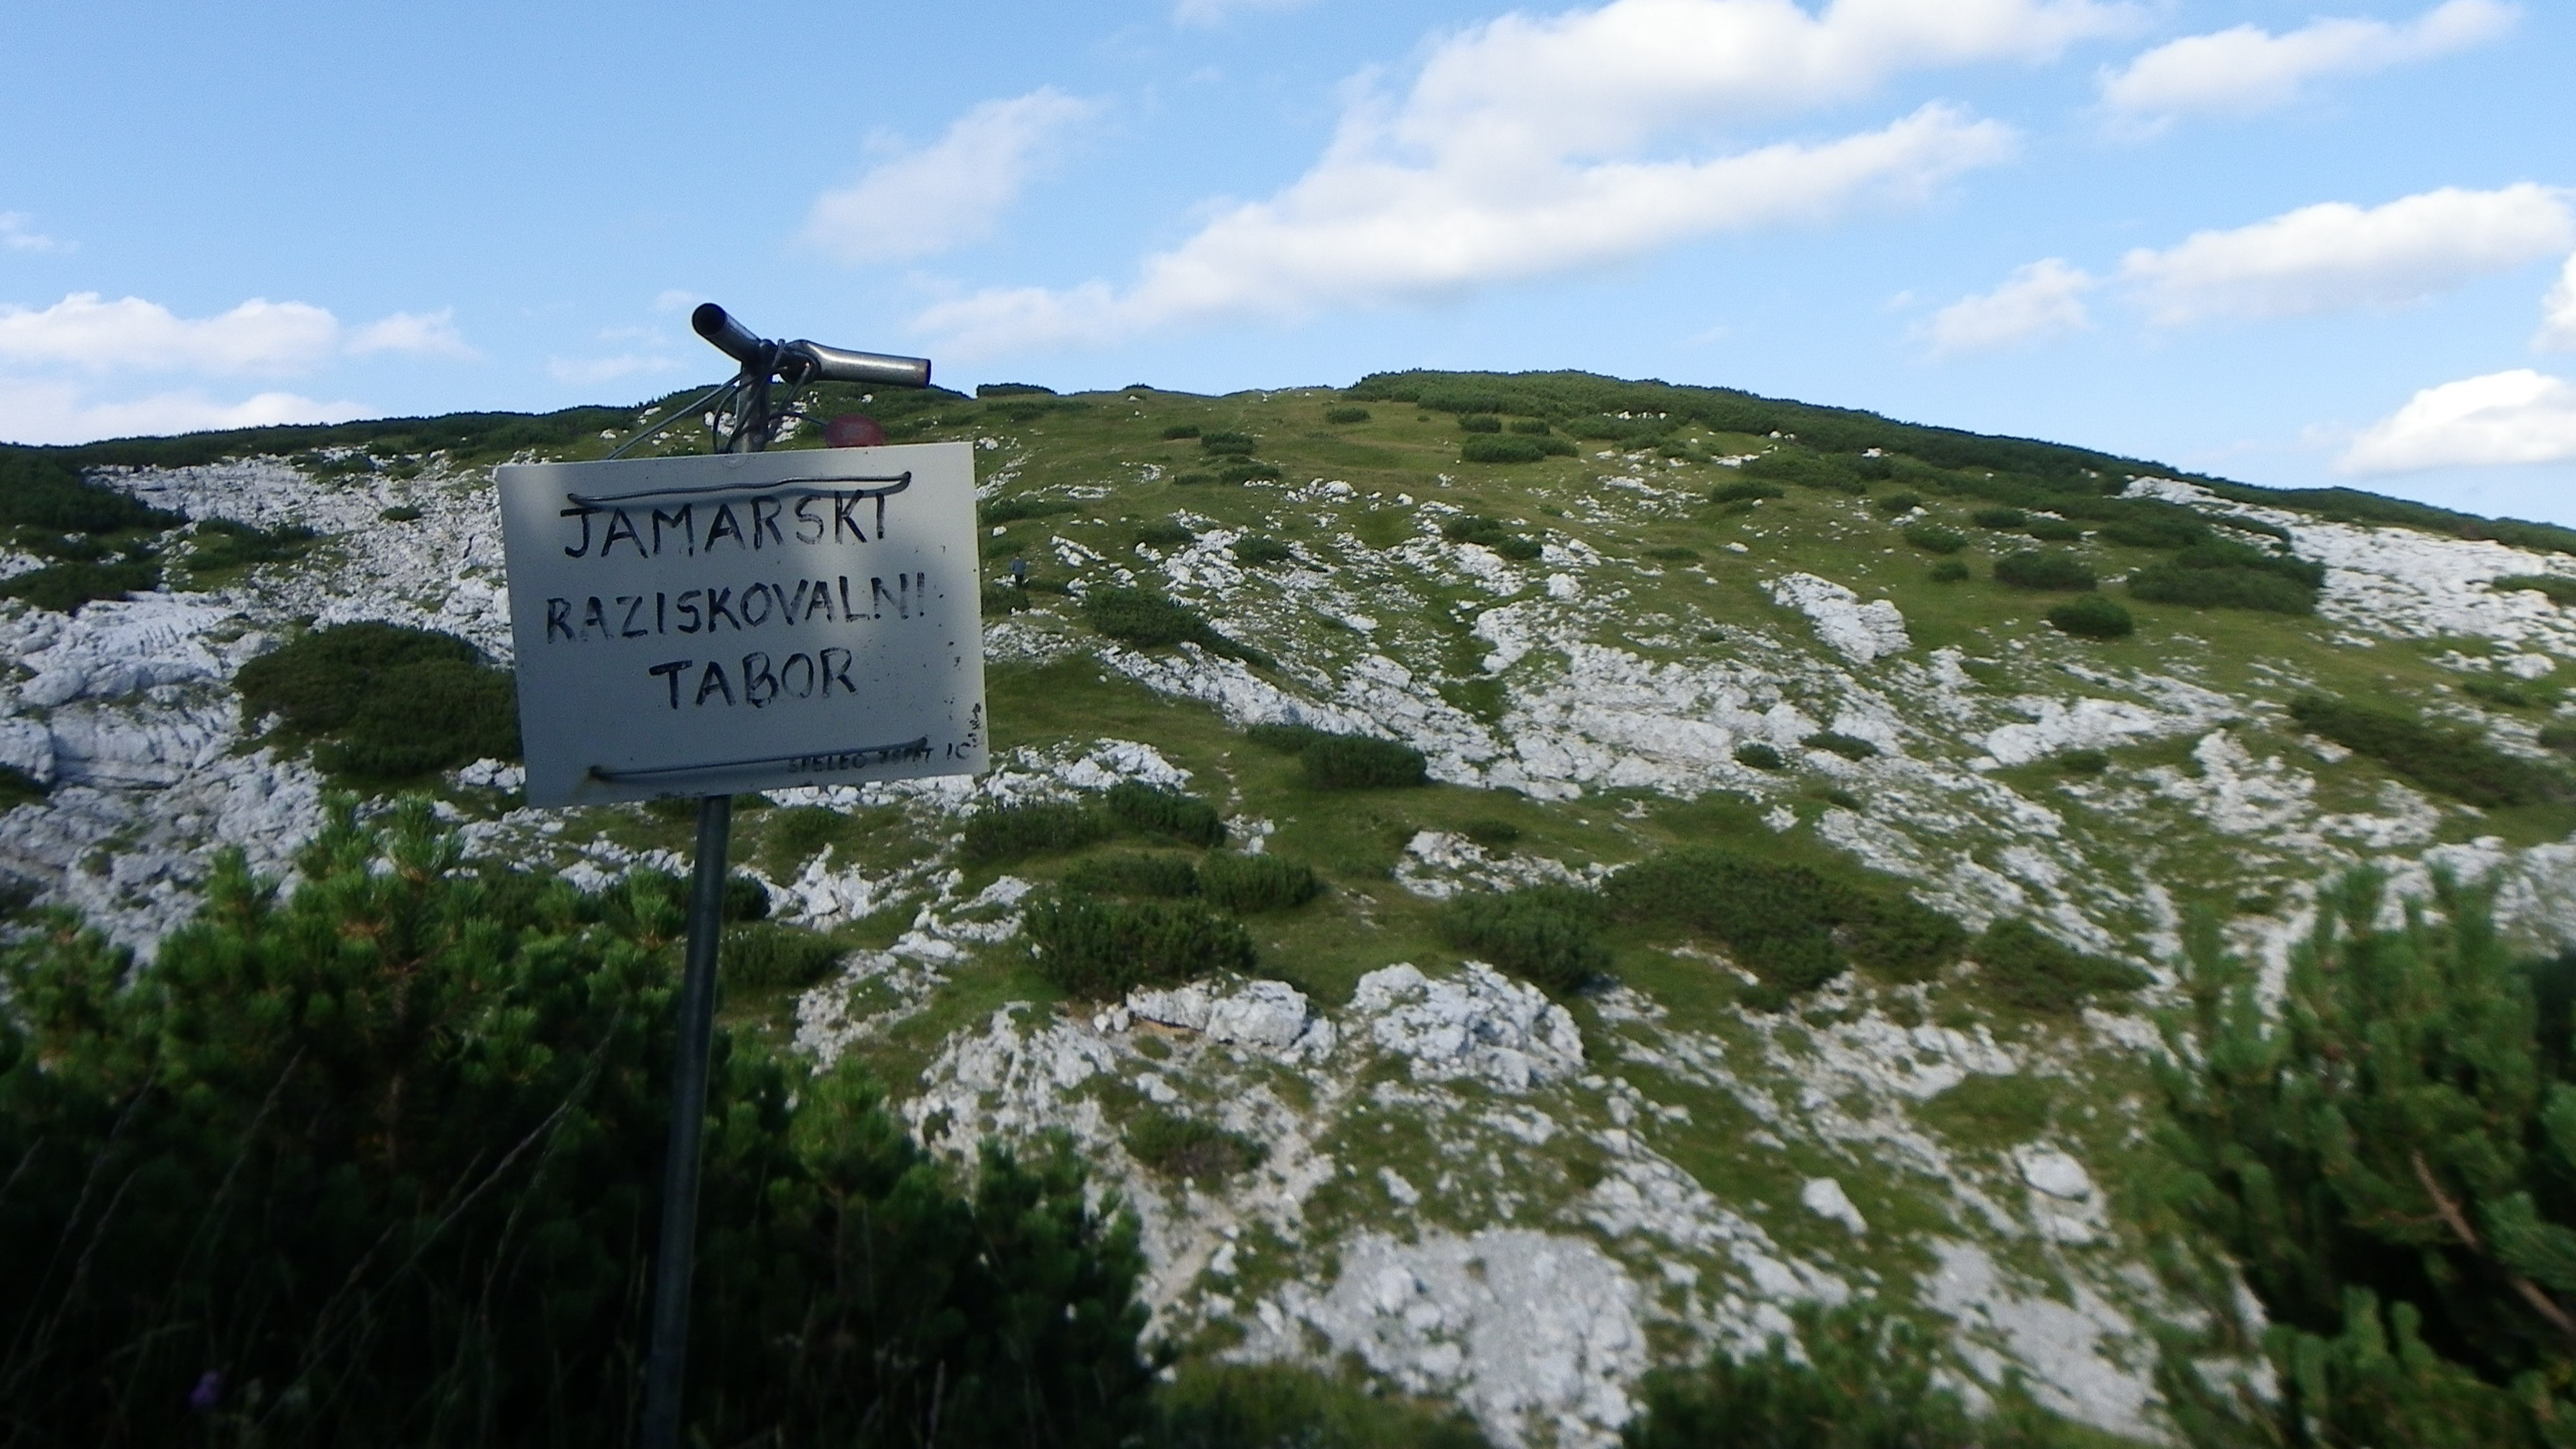
\includegraphics[width = \textwidth]{2012/summary/2012-08-08-19.13.30-Rhys Tyers-Pentax X90-IMGP3418--orig.jpg}
\caption{The campsite sign. \pic{Rhys Tyers}} \label{camp sign}
\end{pagefigure}